% 1000 Henning
\chapter{Modellierung}
\label{cha:Modellierung}

Dieses Kapitel thematisiert die Phase Modeling des ref CRISP-DM Prozesses. Diese Phase hat eine hohe relevanz und wird typischerweise bei Projekten welche CRISP-DM methodisch verwenden mehrfach iteriert quelle. Ziel dieser Phase ist es aus den zuvor vorbereiteten Daten und gewonnen Erkenntnissen einen Mehrwert zu stifen quelle. Im Konkreten Fall sollen die zuvor gesammelten Daten genutzt werden um ein LLM acro in die Lage zu versetzen eine Schätzung zu machen welcher RCA acro quelle vorliegt. Innerhalb des Kapitels werden Ansätze zur Lösung diskutiert, diese sind die Zusammenfassung der verschiedenen Iterationen des durchlaufenen CRISP-dm acro Prozesses. Ebenso werden besondere Herausforderungen sowie erste Erkenntnisse dargestellt, bevor dann im folgenden Kapitel die Qualität der Antworten der verwendeten LLMs qualitativ bewertet werden kann. 

\section{Zielsetzung}
\label{sec:Zielsetzung}

Die Ausgaben aus dem modell sollen nicht nur die Forschungsfrage beantworten (quelle todo src) sondern auch mit den von nezha (src ref) gelieferten Ergebnissen verglichen werden. Da die Ausgabe von nezha aus einer Liste von möglichen RCA auswählt entspricht die durch das LLM zu bewerkstelligende Aufgabe am ehestesten der einer Klassifikation. Nezha trifft in der Ausgabe die folgenden Klassen\footnote{Im acro nezha Framework in file.ext ersichtlich}:

\begin{itemize}
\item exception
\item return
\item cpu contemtion
\item network
\item asdf-
\end{itemize}

Der zu definierende Prompt muss demnach ebenso zu einem sogenannten exact match (EM) führen, die spätere Validierung und Evaluierung des Verfahrens und der Ausgaben muss diese Maßgabe berücksichtigen. Da die bloße Einteilung in diese wenigen Klassen jedoch noch nicht den maximalen Nutzen stiftet wäre grundsätzlich die Erweiterung der Ausgaben über die Klassifizierung hinweg sehr positiv bzw. ach nötig. Dazu wären im Falle von Codebugs (Exceptions und returns) eine Angabe zur Codestelle oder ein Trace denkbar, im Falle von Netzwerk oder CPU-Fehlern eine genaue Angabe des betroffnen PODs, Dienstes oder Hosts.

\section{Datenaufteilung}
\label{sec:datasplit}
Ein normaler Ansatz wäre ein vortrainiertes LLM noch nachzutrainieren tbd rs quelle. Um dieses Nachtraining durchzuführen ist eine Aufteilung der bestehenden Daten in Trainingsdaten, Validierungsdaten und Testdaten oft sinnhaft qquelle. Konkret ist das in den verwendete Daten set tbd aus nezha ist frei verfügbar, es beinhaltet in der bereinigten, vorverarbeiteten Version ~112 Records, dem liegen 56 injezierte Fehler zugrunde. Typisch ist eine herangehensweise mit einer 70-20-10 Aufteilung, wobei die Aufteilung mit 70\% Trainingsdaten, 10\% Validierungsdaten und  20\% Testdaten (prüfen quelle) für viele Anwendungsfälle passend ist. Im vorliegenden konkreten Fall ist jedoch Wie bereits in  (ref Understanding) dargestellt, leider nur ein vergleichsweise geringer Datenbestand verfügbar. Ein Training auf diesen Bestand nach der vorher gezeigten Aufteilung ist als wenig stabil zu bewerten (quelle). Um eine Art Datenaufteilung dennoch auszuführen wurden im Rahmen der Versuche zum Modeling die Verfahren Few-shot und One-shot angewandt. Beide basieren darauf [Erklärtext, ggf. ref theorie] mit weniger bzw., fast keinen Daten ein Retraining durchzuführen. Im Ergebnis konnten die besten Resultate erzielt werden wenn kein Nachtraining erfolgte. Da dieser Datenbestand zu klein ist um ein sinnhaftes Training für ein LLM durchzuführen quelle, musste eine andere Methodik zum EInsatz kommen, das gewählte Verfahren wird als Zero-Shot Prompting bezeichnet, nähere Ausführungen dazu unter \autoref{sec:prompte}
 

\section{Promptengineering}
\label{sec:prompte}
Wie zuvor dargestellt sollen die vorverarbeiteten Daten an ein LLM gegeben werden (ref). Dies geschieht typsischerweise mittels eines sogenannten Prompts, dies ist in den meisten Fällen eine textbasierte eingabe (quelle). Im konkreten Fall soll diese Eingabe nicht interaktiv sondern mittels API (acro) durch ein Programm erfolgen. Um die gemachten Eingaben zu optimieren bedarf es Methoden und Instrumente des Prompt-engineering. Ziel ist, die Prompts so zu gestalten, das möglichst nützliche, spezifische und qualitativ verwendare Ausgaben durch das LLM generiert werden. Grundsätzlich gilt beim Entwerfen von Prompts, egal über welchen Weg sie an ein LLM gerichtet werden, das sie natürlichsprachlichen zu besseren Ergebnissen\autocite{Brown2020}[S. 3] führen, unnötig technisch oder abstrakte Promts führen demnach zu schlechteren Ergebnissen. 

Ein Blick in die Literatur offenbart eine Vielzahl von möglichen Techniken zu Promptgestaltung und optimierung. quelle Listet etwa 29 Techniken, kategoriesiert in 12 Anwendungsbereiche\autocite[S. 3]{Sahoo2024}. Die Techniken folgen in der Regel gewisser Methodik und Denkmustern, sie schließen sich teilweise auch auch aus, es galt also zum konkreten Anwendungsfall passende Techniken auszuwählen. Dem Thread of Thought (ThoT) acro Ansatz, beschrieben in quelle \autocite{Zhou2023}, wurde sich dabei angenähert. Dieser Ansatz beschreibt ein zunächst chaotischen Kontext schritt weise zu nähern, iterativ zu verfeinern und die Ergebnisse mittels sogenanntem Exact Match (quelle acro em) zu messen. Thot zeigt in Experimenten das es ein verbessertes Schlussfolgern aufweist, dies ist insbesondere im hier vorliegenden Anwendungsfall, dem finden einer ursprünglichen Fehlerursache von essentieller Bedeutung. Die gesteigerte Schlussfolgerungsqualität wird auch in einer ähnlich gelagerten Arbeit von \autocite{Wei2022}[S. ?] dargestellt. Bereits nach wenigen Versuchen konnte programmatisch ein verwertbares Ergebnis erzielt werden, dies spricht zum einen für eine leichte Handhabbarkeit von LLMs (acro) via python über API als auch über die Wirkungsmächtigkeit der angwandten Methodik über Thot (acro). Mehrere Techniken wie x und y quelle, bedingen z.B. ein komplexes Retraining, welches wie bereits in \autoref{sec:datasplit} bedingt durch die geringe Datenmenge kaum sinnhaft möglich war.

Wie bereits in \autoref{sec:datasplit} beschrieben wurde Zero-shot Learning eingesetzt, obwohl der Literatur nach ein Few-Shot Verfahren signifikant bessere Ergebnisse erzielen sollte\autocite{Brown2020}[S.4]. Ursachen für diese nicht vorhergesehene Feststellung könnten darin liegen das \citeauthor{Brown2020} in Ihrer Forschung noch auf ChatGPT 3\footnote{Für den Aufbau des Prompts dieser Arbeit wurde ChatGPT 4 verwendet.} bezogen haben oder ggf. auch aus der Qualität oder Quantität der zugrundeliegenden Daten.

Der finale, optimierte Prompt ist in \autoref{fig:finalprompt} erstlich. Die mit den geschweiften Klammern gekennzeichneten Begriffe sind wie Variablen zu sehen und werden zur Laufzeit durch den aufrufenden code gefüllt. Quelle der eingesetzten Variablen sind die vorverarbeiteten Daten aus \autoref{quelle vorverarbeitung}. 

\begin{figure}
    \centering
    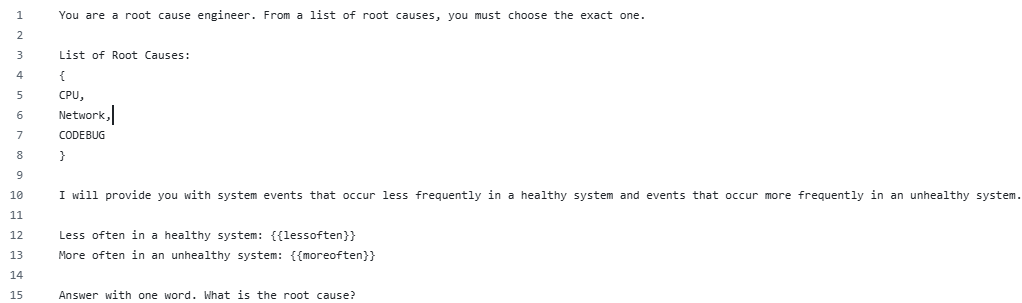
\includegraphics [width=0.5\linewidth] {bilder/finalprompt.png}
    \caption [Finaler, optimierter Prompt]{Finaler, optimierter Prompt. Quelle: eigene Darstellung}
    \label{fig:finalprompt}
\end{figure}
%ggf noch von https://github.com/virsel/ba_anw_promptfoo einfügen, Rückfrage ob relevant! quelle todo! 




Folgt man den Ausführungen zum Promptengineering von quelle sind dazu folgende Punkte beachtenswert:

Few-Shot Prompting: Das Modell erhält wenige Beispiele innerhalb des Prompts, um die gewünschte Aufgabe zu verstehen und auszuführen. Dies verbessert die Genauigkeit, indem es dem Modell Kontext und Struktur für die erwartete Antwort bietet. 




TODO:
Rechtschreiber!!
1-2 Bilder
Inhalt eindampfen?
Ggf. noch Zeroshot besser belegen
Inhaltliche AUfteilung mit 3 sections nur wenn noch wörter gebraucht werden
